
\chapter{Le contexte}
 %% : l'outil de déploiement du jeu en ligne
\section{Architecture de l'écosystème Mamba Nation}

\subsection{Architecture Générale}

Mamba Nation est composé de trois couches : La couche utilisateur, la couche
Game Server aussi appelée ``La Nation'', et la couche Back-Office.

La couche utilisateur est composée de l'application Facebook, l'applet qui
affiche le monde Mamba Nation en 3D, un site web, un forum et une application
IPhone appelée Battle.
L'applet est responsable du rendu 3D du jeu.

La Nation regroupe un ensemble de composants applicatifs qui donnent vie au
monde de la Nation: moteur du Jeu, base de données, etc.. Des Web services sont
aussi utilisés pour permettre aux partenaires externes d'accèder à la Nation. 
Le service ``Event log'' est un composant qui collecte les événements
utilisateurs.

La couche Admin est composée de la BI (Business Intelligence Platform) qui
produit un grand ensemble de KPI (Key Performance Indicator) du jeu et un outil
Back-Office pour que le jeu puisse être géré par les équipes Operation.

\subsection{Diagramme Fonctionnel}

Le diagramme représente les principaux services fonctionnels de Mamba Nation.
Ces services peuvent être organisés en trois couches :
\begin{itemize}
\item couche User: services accesibles directement par l'utilisateur final
\item couche Game: moteur du jeu, les services pour les partenaires externes et les
  composants internes
\item couche Admin: reporting et outils de gestion
\end{itemize}

\begin{figure}[H]
  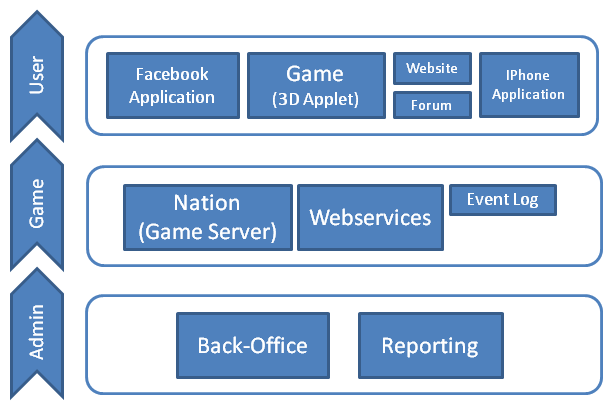
\includegraphics[scale=0.75]{MN-functional-diagram.png}  
  \caption{Diagramme fonctionnel de la Nation}
\end{figure}

\subsection{Architecture Technique}

La Nation contient les services de base de Mamba Nation. Ça inclut le Game
Server, le moteur d'applet 3D, l'application facebook, les services web et le
site web.

La Nation utilise aussi un ensemble de services techniques :
\begin{itemize}
\item Zookeeper : service centralisé pour maintenir les informations de configuration
\item Route 53 : service Web de système de noms de domaine (DNS)
\item Mongo DB: base de données orientée document
\item RabbitMQ : solution de messagerie orientée messages pour créer un réseau
  d'échange d'informations entre des applications.
\item RDS: base de données MySql fournie par Amazon
\item Jetty: moteur de servlet basé sur Java
\item Apache: héberge le site php
\item S3 : plateforme de stockage ``illimité''
\end{itemize}

Les utilisateurs se connectent au Game Server à travers les dispatchers qui ont la
responsabilité de gérer les connections TCP.

La plupart des services sont développés avec le langage Scala ce qui facilite le
développement d'applications évolutives.

Le site web est développé en PHP avec un serveur Zend et un cache APC. Il est
déployé sur Apache.

\begin{figure}[H]
  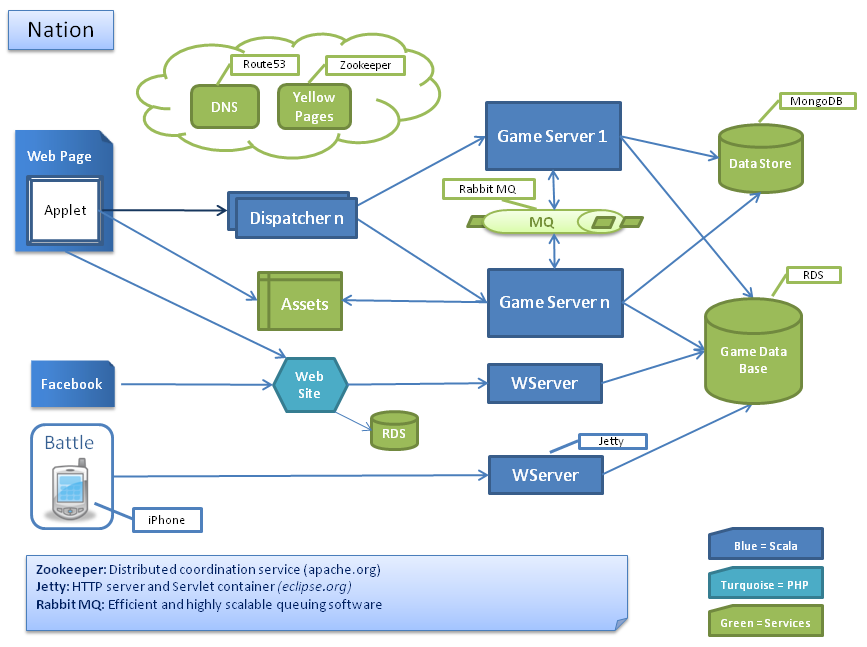
\includegraphics[scale=0.75]{MN-technical-diagram.png}  
  \caption{Diagramme technique de la Nation}
\end{figure}

\subsection{Statistiques du Jeu}

\begin{figure}[H]
  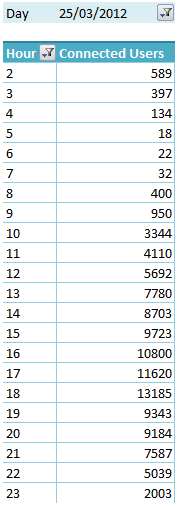
\includegraphics[width=0.20\textwidth]{connected-users-diagram.png}
  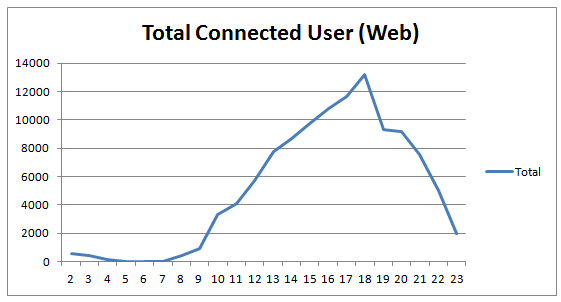
\includegraphics[width=0.80\textwidth]{connected-users-graph.png}
  \caption{Diagramme du nombre d'utilisateurs connectés dans la journée du 25 mars 2012}
\end{figure}

\section{L'outil d'infra : un outil pour déployer le jeu}

Les ingénieurs de l'équipe \textit{infrastructure} ont conçu un outil en ligne
de commande pour déployer une infra.
Chaque équipe de l'entreprise utilise cet outil pour gérer leur propre
infrastructure. Par exemple, l'équipe \textit{engine} utilise cet outil de
déploiement pour gérer leur infrastructure \textit{engine}.

Un développeur de l'équipe \textit{engine} peut exécuter la commande
\textit{status engine} pour se renseigner sur l'état de son infra. L'outil en
ligne de commande affiche :
\begin{verbatim}
    engine_all_0 (i-51e60a18 / 54.247.21.95)        :       running
    Instance reachability check passed 
    System reachability check passed
\end{verbatim}
Tout va bien, l'instance \verb?engine_all_0? est bien en train de s'exécuter.

\section{Le concept de Promises}

L'outil d'infra utilise le concept de Promises partout dans son code.

Les \textit{Promises} fournissent un bon moyen de raisonner sur l'exécution de
nombreuses opérations en parallèle - d'une façon efficace et non bloquante.

L'idée est simple, une Promise est une sorte de conteneur d'objet que l'on peut
créer pour un résultat qui n'existe pas encore.

Généralement, le résultat d'une \textit{Promise} est calculé de manière
concurrente et peut être récupéré plus tard.
Composer des tâches concurrentes de cette manière permet d'avoir du code
parallèle non bloquant, asynchrone plus rapide.

Une Promise est une abstraction qui représente une valeur qui peut devenir
disponible à un certain point.
Un objet Promise contient soit le résultat d'un calcul soit une exception dans
le cas où le calcul a échoué.
Une propriété importante d'une Promise est qu'elle est immuable; le détenteur de
la Promise ne peut à aucun moment modifier la valeur qu'elle contient.

Voici un exemple de création d'une Promise qui appelle une méthode asynchrone
getUsers. Le résultat devient disponible une fois que la Promise se termine.
\lstset{language=scala,
  frame=single                   % adds a frame around the code
}
\begin{lstlisting}
  val usersProm: Promise[List[Users]] = Promise {
    session.getUsers
  }
\end{lstlisting}

Nous pouvons chaîner les calculs sur la Promise de base en utilisant la méthode
map qui reçoit une fonction en paramètre. 
\begin{lstlisting}
  val alexProm: Promise[User] = usersProm.map { users => users.filter(_.name == ``Alex'').head }
\end{lstlisting}

Une fois tous les calculs effectués sur notre Promise, nous pouvons récupèrer sa
valeur de façon bloquante (waitAndGetEither) ou non bloquante (mapEither).
Récupération de l'utilisateur Alex de façons bloquante :
\begin{lstlisting}
val alex:User = alexProm waitAndGetEither() match {
    case Right(alex: User) => alex
    case Left(t: Exception) => t.printStackTrace(); throw t
  }
\end{lstlisting}
Si la Promise s'est terminée avec succès alors la méthode waitAndGetEither
renvoie une instance Right qui contient notre utilisateur Alex.
Si l'une des fonction passée aux différentes Promises de la chaîne a échouée, la
méthode waitAndGetEither renvoie une instance Left qui contient l'exception
lancée.

\section{L'outil d'infra et AWS}

L'outil d'infra utilise l'API Java AWS pour :
\begin{itemize}
\item créer, supprimer une instance
\item récupérer le status d'une instance
\item démarrer, arrêter une instance
\item créer, supprimer un groupe de sécurité
\item authoriser des IP et ports sur un groupe de sécurité
\item lister les groupes de sécurité
\end{itemize}

\section{L'outil d'infra et Chef}

Toutes les informations concernant une infra sont stockées dans Chef.
Lors de la création d'une infra, l'outil en ligne de commande stocke entre
autres le nom de l'infra, la région AWS, le nom de la base de données et le nom
du groupe de sécurité dans un Databag Chef.

L'outil d'infra utilise l'API REST de Chef pour récupèrer des informations ou
effectuer des actions. 

\section{Usage}

L'outil d'infra en ligne de commande reçoit en entrés un nom de commande
et ses arguments. Si la commande n'existe pas, l'outil d'infra affiche l'aide
d'usage.
Voici l'affichage de l'aide, on peut y voir toutes les commandes disponibles :
\begin{verbatim}
Usage: infra <cmd> [<infra>] [<file>] [<key>=<value>]*

    Infra admin tool config file:
      Config parameters must be specified in the 'infra.conf' file located in the 'config' directory.
      It should contain one <field>=<value> definition per line.

    Infra creation, pass config file:
      create <file>
        Create an infrastructure as defined in the given config file.
     migrate <file>
        Migrate databases for a particular environment in an infrastructure as
        defined in the given config file.


    Infra management, pass infra:
      start <infra>
        Start the given infrastructure.
      stop <infra>
        Stop the given infrastructure.
      status <infra>
        Show status of the given infrastructure.
      destroy <infra>
        Destroy the given infrastructure.

    Service management, pass infra:
      start-services <infra>
        Start services on the given infrastructure.
      stop-services <infra>
        Stop services on the given infrastructure.
      restart-services <infra>
        Restart services on the given infrastructure.
      status-services <infra>
        Show status of the services on the given infrastructure.

    Database management, pass infra:
      deploy-db <infra>
        Run the 'deployDb' command on the given infrastructure.
      liquibase-install <infra>
        Run the 'liquibase-install' command on the given infrastructure.
      liquibase-sync <infra>
        Run the 'liquibase-sync' command on the given infrastructure.
      liquibase-update <infra>
        Run the 'liquibase-update' command on the given infrastructure.
      run-migration-tool <infra>
        Run the 'run-migration-tool' command on the given infrastructure.

    Text management, pass infra :
      deploy-wti <infra>
        Export the last texts from WTI on amazon S3 ; to really use them you
        have to modify the file "launch.js.php" on the "a" environment.


    Environment management, pass infra and optionally updated values:
      show <infra> [<key>]*
        Show the "a" environment on the given infrastructure.
      update-env <infra> <file>
        Update the "a" environment on the given infrastructure as defined in the given config file.
      update-env <infra> [<key=value>]*
        Update the "a" environment on the given infrastructure as defined in the key-value arguments.

    Various utilities, rarely used:
      list
        List all infrastructures.
      start-all
        Start all infrastructures and all services.
      stop-all
        Stop all infrastructures.
      register-dns <infra>
        Register DNS records for the given infrastructure.
      switch-dns <infra>
        Switch LIVE dns to point to the given infrastructure.
      export <infra>
        Export the databag item describing the given infrastructure from the Chef server to a file.
      import <infra>
        Import the databag item describing the given infrastructure from a file to the Chef server.
      export-databags
        Export all databags from the Chef Server to the file system.
      import-databags
        Import all databags from the file system to the Chef Server.
\end{verbatim}

